\begin{figure}[!t]
\centering
%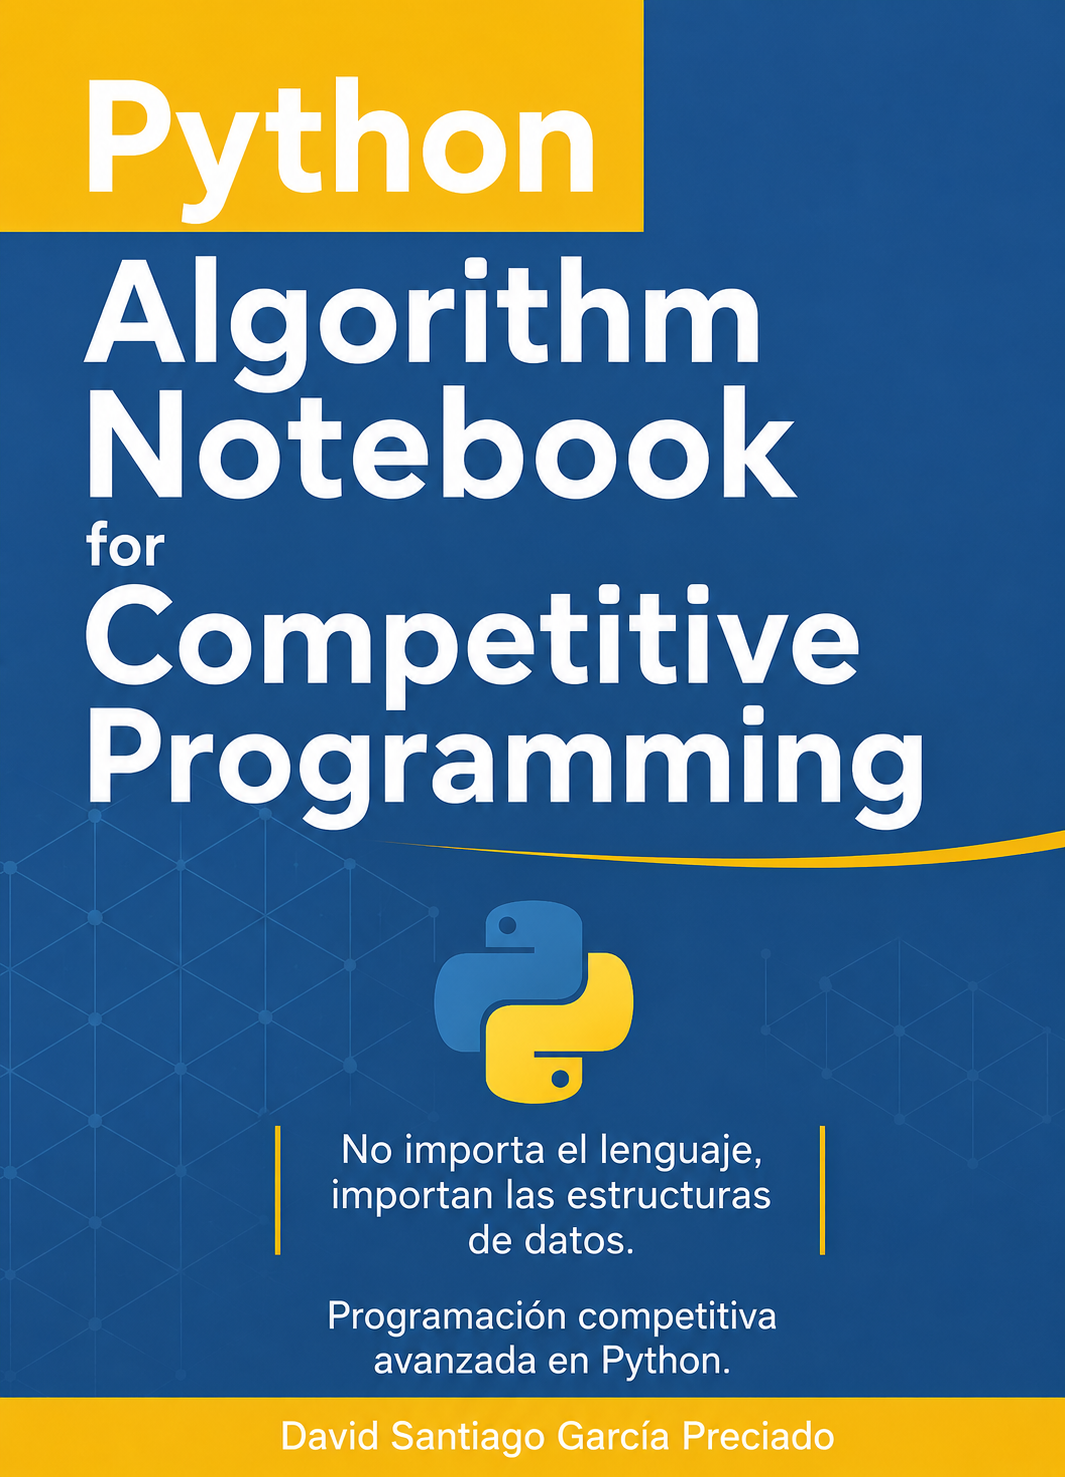
\includegraphics[width=\linewidth]{images/image1.png}
\end{figure}

Este Notebook tiene una estructura simple. 
Hay preguntas guía para reconocer cuándo aplica el algoritmo, para qué sirve, su complejidad, el fundamento teórico, y un ejercicio real resuelto con esa técnica. 
